\documentclass[a4paper]{article}

\usepackage[fontset=fandol]{ctex}
\usepackage{amsmath, amssymb}
\usepackage{graphicx}
\usepackage[margin=2.3cm]{geometry}
\usepackage[most]{tcolorbox}
\usepackage{etoolbox}
\usepackage{listings}
\usepackage{hyperref}
\usepackage{booktabs}
\usepackage{subcaption}
\usepackage{float}
\usepackage{tikz}
\IfFileExists{pgfplots.sty}{
    \usepackage{pgfplots}
    \pgfplotsset{compat=1.18}
}{}

\newtcolorbox{knowledgebox}[1]{
    enhanced, colback=blue!5!white, colframe=blue!75!black, colbacktitle=blue!75!black,
    coltitle=white, fonttitle=\bfseries, title=#1, attach boxed title to top left={yshift=-2mm, xshift=2mm},
    boxrule=1pt, sharp corners
}

\newtcolorbox{importantbox}[1]{
    enhanced, colback=yellow!10!white, colframe=yellow!80!black, colbacktitle=yellow!80!black,
    coltitle=black, fonttitle=\bfseries, title=#1, sharp corners
}

\newtcolorbox{warningbox}[1]{
    enhanced, colback=red!5!white, colframe=red!75!black, colbacktitle=red!75!black,
    coltitle=white, fonttitle=\bfseries, title=#1, sharp corners
}

\lstset{
    language=Python,
    basicstyle=\ttfamily\small,
    keywordstyle=\color{blue},
    stringstyle=\color{red!60!black},
    commentstyle=\color{green!60!black},
    breaklines=true,
    frame=single,
    numbers=left,
    numberstyle=\tiny\color{gray},
    captionpos=b,
    extendedchars=false
}

\newcommand{\notetitle}{CS336 语言模型从零构建：从 Tokenization 到 RLVR 的统一讲义}
\newcommand{\noteauthors}{Codex 基于 Stanford CS336 2025 课程视频与官方课件整理}
\newcommand{\notedate}{2026-04-06}
\newcommand{\videochannel}{Stanford Online}
\newcommand{\videopublishdate}{Spring 2025}
\newcommand{\videoduration}{17 讲，约 22.32 小时}
\newcommand{\videourl}{https://www.youtube.com/playlist?list=PLoROMvodv4rOY23Y0BoGoBGgQ1zmU_MT_}
\newcommand{\videocoverpath}{../raw/00_PLoROMvodv4rOY23Y0BoGoBGgQ1zmU_MT_/00_PLoROMvodv4rOY23Y0BoGoBGgQ1zmU_MT_.jpg}

\begin{document}

\begin{titlepage}
\centering
{\Large 课程笔记\par}
\vspace{1.2cm}
{\huge\bfseries \notetitle\par}
\vspace{0.8cm}
{\large \noteauthors\par}
\vspace{0.3cm}
{\large \notedate\par}
\vspace{1.2cm}

\ifdefempty{\videocoverpath}{
{\small 请在生成笔记时填入视频封面图的本地路径。\par}
}{
\includegraphics[width=0.82\textwidth,height=0.45\textheight,keepaspectratio]{\videocoverpath}\par
}

\vfill
\begin{tcolorbox}[width=0.9\textwidth, colback=black!2!white, colframe=black!60, sharp corners]
\textbf{视频作者/频道}：\videochannel\par
\textbf{发布日期}：\videopublishdate\par
\textbf{视频时长}：\videoduration\par
\textbf{视频链接}：
\ifdefempty{\videourl}{
未填写
}{
\href{\videourl}{\nolinkurl{\videourl}}
}
\end{tcolorbox}
\end{titlepage}

\tableofcontents
\newpage

\section{课程导论与语言模型全景}

\subsection{讲次 1：为什么要从零构建语言模型}
CS336 的出发点不是“再讲一遍 Transformer”，而是对当下研究生态的一个反拨：越来越多研究者只和封装好的接口打交道，却不再真正理解模型是如何被数据、算力、优化器与系统共同塑造出来的。课程的核心立场可以压缩成一句话：\textbf{想做真正有穿透力的研究，就需要把整条语言模型流水线重新搭起来一次。}

从课程开场就能看到两条张力。第一条张力是\textbf{工业化}：前沿模型规模越来越大，训练成本越来越高，公开细节越来越少。第二条张力是\textbf{可迁移性}：小模型和大模型之间并不完全同构，但仍然有三类知识是可以迁移的，即机制层知识、系统化思维方式，以及对设计权衡的直觉。

\begin{importantbox}{本课最核心的认知框架}
这门课真正想教的，不是“照着配方复刻一个小模型”，而是学会在固定资源约束下，系统性地问：数据应该怎么选，token 应该怎么切，架构应该怎么改，训练应该怎么配，比起盲目堆规模，哪里还能提升效率。
\end{importantbox}

\begin{knowledgebox}{三类可迁移知识}
\textbf{Mechanics} 关注模型怎样运作，比如注意力、KV cache、并行通信。\par
\textbf{Mindset} 关注面对真实资源约束时怎样思考，比如 roofline、scaling law、通信开销。\par
\textbf{Intuitions} 关注经验性设计，如数据配比、激活函数、MoE 路由与训练稳定性。
\end{knowledgebox}

\begin{figure}[H]
\centering
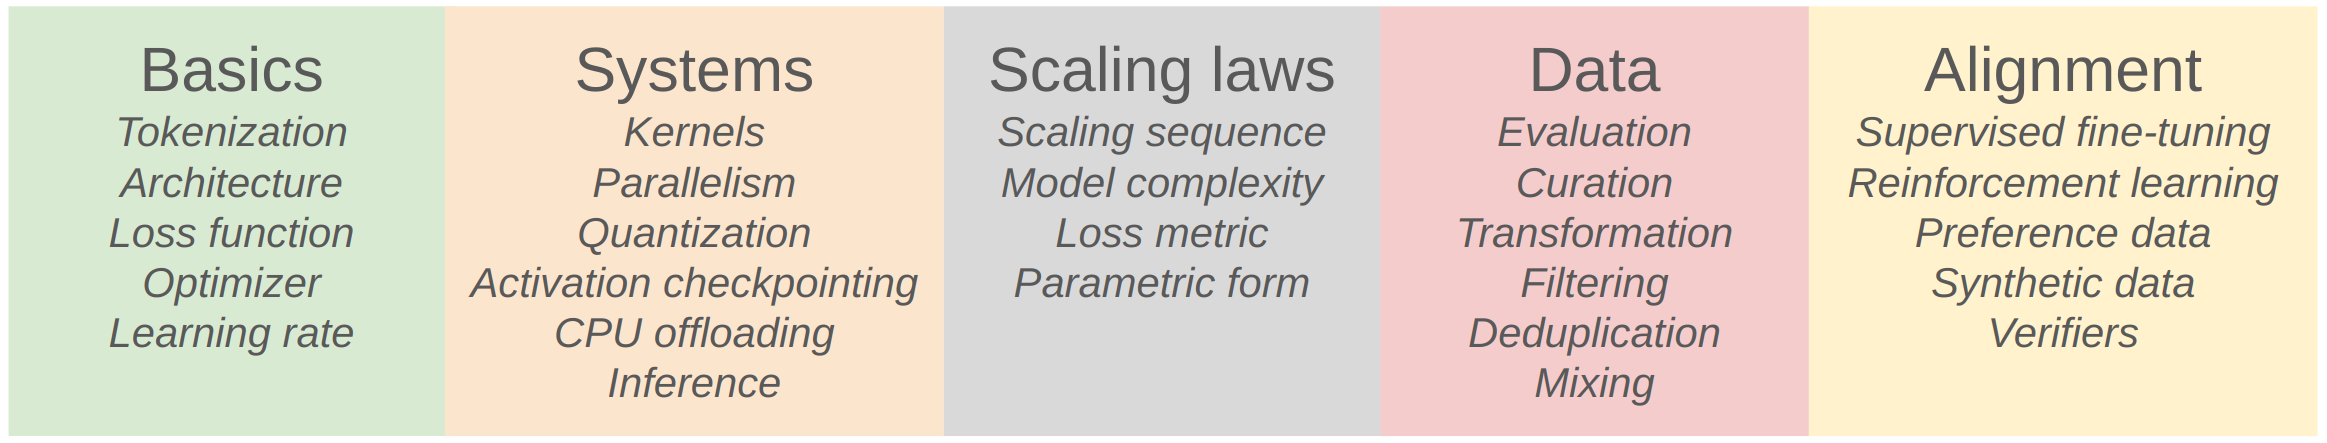
\includegraphics[width=0.9\textwidth]{../materials/spring2025-lectures/images/design-decisions.png}
\caption{CS336 把语言模型训练看成一连串设计决策：数据、tokenization、架构、训练、系统与对齐缺一不可。}
\end{figure}

\subsection{讲次 1：从课程地图看整条 LM 流水线}
课程把“从零构建语言模型”拆成了一个非常完整的工程闭环：先做 tokenization 和基础架构，再做资源核算、GPU 与 kernel 优化、并行训练、推理系统、scaling laws、评测、数据工程，最后走到 SFT、RLHF 与 RLVR。一个重要的教学设计是：\textbf{后面的所有高级主题都不是孤立技巧，而是在前面基础模块之上自然长出来的。}

例如，tokenization 看起来只是预处理问题，但它会影响序列长度，从而影响训练 FLOPs、KV cache、推理吞吐和数据利用率；并行训练看起来是系统问题，但其实又反过来决定了哪些架构在大规模上更现实；对齐看起来是后训练问题，但它又依赖推理系统是否足够高效、评测体系是否足够可靠。

\begin{warningbox}{不要把课程拆成互不相干的专题}
如果把 CS336 只看成“Transformer + GPU + RLHF”的松散集合，很容易学一堆局部技巧却看不到统一目标。课程真正的主线是：\textbf{如何在给定资源约束下，把原始文本变成高质量、可控、可部署的语言模型。}
\end{warningbox}

\subsection{讲次 1：Tokenization 为什么仍然是必要之恶}
第一讲最后回到 tokenization，本质问题很朴素：语言模型通常以离散 token 为基本对象，但真实世界中的输入却是 Unicode 字符串，因此系统必须提供双向映射：字符串编码成 token 序列，token 序列再解码回字符串。课程并不把 tokenization 神秘化，而是把它看成工程折中。

从课程视角看，字符级、词级和纯字节级方案都各有缺陷。词级词表太脆弱，字符级序列太长，字节级虽然概念上最干净，但在当前主流架构与算力条件下通常又不够计算友好。因此 BPE 之类的子词方案，本质上是用语料统计把“高频片段”变成中间粒度的离散符号，用更合适的序列长度换取更好的训练与推理效率。

\begin{figure}[H]
\centering
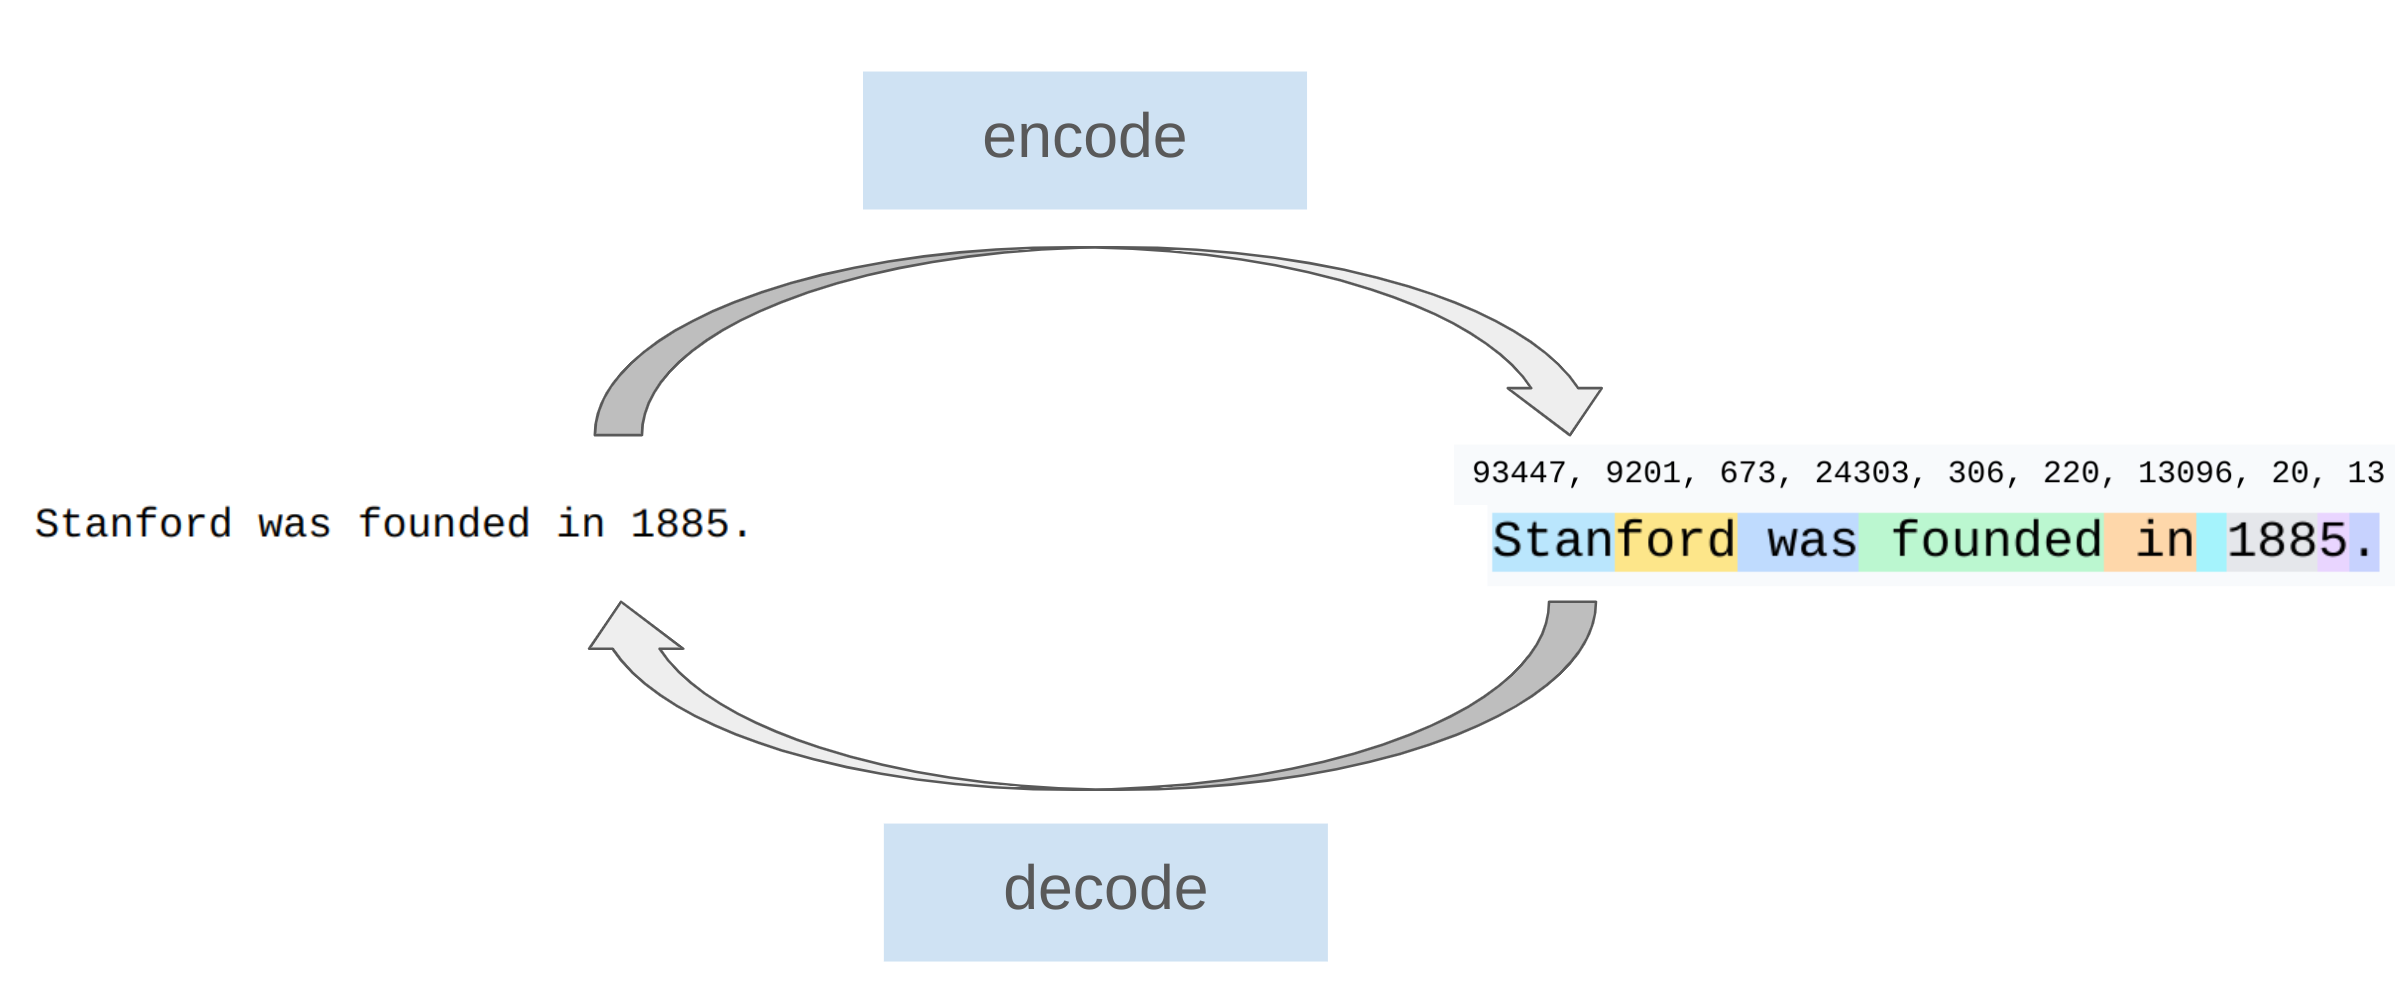
\includegraphics[width=0.78\textwidth]{../materials/spring2025-lectures/images/tokenized-example.png}
\caption{Tokenization 的核心不是“把文本切碎”，而是在表达能力、序列长度与计算代价之间找一个对整个系统最有利的折中。}
\end{figure}

\subsection{本章小结}
课程第一讲完成了两个奠基动作：一是说明为什么今天仍然值得“从零理解”语言模型，二是给出整门课的统一路线图。它把整个问题压缩成一个资源优化问题：在有限的数据、硬件与时间预算下，如何做出最好的模型。tokenization 则是这条流水线的第一个具体决策点。

\section{工程起点：PyTorch 与资源核算}

\subsection{讲次 2：为什么资源核算是语言模型工程的起点}
第二讲最重要的态度转变是：\textbf{写模型代码之前，先学会记账。} 课程把资源拆成了两种最基本的账本：内存账本与计算账本。前者回答“这次训练能不能塞进硬件里”，后者回答“这次训练到底贵在哪里”。

内存账本至少要区分参数、梯度、主权重与优化器状态。一个看起来只是“参数量为 $N$” 的模型，在真实训练时往往远不止存一份权重，尤其在 Adam 一类优化器下，内存消耗会被多份状态显著放大。精度选择也因此不是表面上的数值问题，而是会直接改变硬件可承载模型规模的问题。

\subsection{讲次 2：精度、显存与 FLOPs}
课程依次讨论了 float32、float16、bfloat16 乃至更低精度格式。直觉上，位宽变小能节省显存、提升吞吐，但代价是数值稳定性更脆弱。CS336 的重点不是背每种格式的标准，而是理解它们在训练中的角色分工：哪些量可以低精度存，哪些量需要更高精度累计，为什么同样一块 GPU，在不同精度策略下可训练模型规模会差很多。

在计算账本上，课程把 FLOPs 视为一种统一尺度，用来比较不同模型设置、不同训练配置的代价。更重要的是，课程强调\textbf{“FLOPs 不是 runtime，但它是第一层近似”}：很多设计先要过 FLOPs 这一关，随后再结合 memory bandwidth、kernel 实现与通信开销判断真实速度。

\[
\mathrm{MFU} = \frac{\text{模型实际完成的 FLOPs/s}}{\text{硬件理论峰值 FLOPs/s}}
\]

其中：
\begin{itemize}
\item $\mathrm{MFU}$：Model FLOPs Utilization，衡量训练是否把硬件真正喂饱。
\item 分子：真实训练过程中由模型前向与反向贡献的有效计算吞吐。
\item 分母：对应 GPU 的理论峰值算力。
\end{itemize}

\begin{importantbox}{MFU 的真正意义}
MFU 不是一个“越大越好”的炫技指标，而是连接算法与系统的桥。它能帮我们区分：到底是模型本身算得不够多，还是 kernel / data loader / 通信让硬件闲着。
\end{importantbox}

\subsection{讲次 2：用小模型练会大模型的会计方法}
第二讲还有一个很关键的工程思想：虽然学生在作业里训练的是小模型，但会计方法必须从一开始就和大模型对齐。也就是说，哪怕当前只在几块卡上跑 TinyStories，你也要知道如果参数扩大一个数量级，内存、吞吐、梯度同步和训练时间会如何变化。

这正是 CS336 不同于“入门深度学习课”的地方。它不是鼓励学生把小实验做通就结束，而是要求你从一开始就用大规模训练者的视角来理解 PyTorch 程序：每个 tensor 的生命周期是什么，参数更新时显存里到底放着什么，瓶颈到底在算还是在搬。

\subsection{本章小结}
第二讲的核心贡献，是把“训练语言模型”从一种模糊的软件实践，变成一种可核算、可预测的工程活动。精度、显存、FLOPs 与 MFU 共同构成了后面 GPU、kernel、并行与 scaling law 各章的共同语言。

\section{架构设计：Transformer 及其变体}

\subsection{讲次 3：现代 Transformer 的共同骨架}
第三讲做的不是再教一次“原始 Transformer”，而是把 2024--2025 年主流大模型架构中真正稳定下来的共性抽出来。课程给出的经验结论非常清晰：现代语言模型整体上越来越向 \textbf{LLaMA-like} 设计靠拢，尤其是在 pre-norm、RoPE、SwiGLU、RMSNorm 与去 bias 化这些选择上。

\begin{figure}[H]
\centering
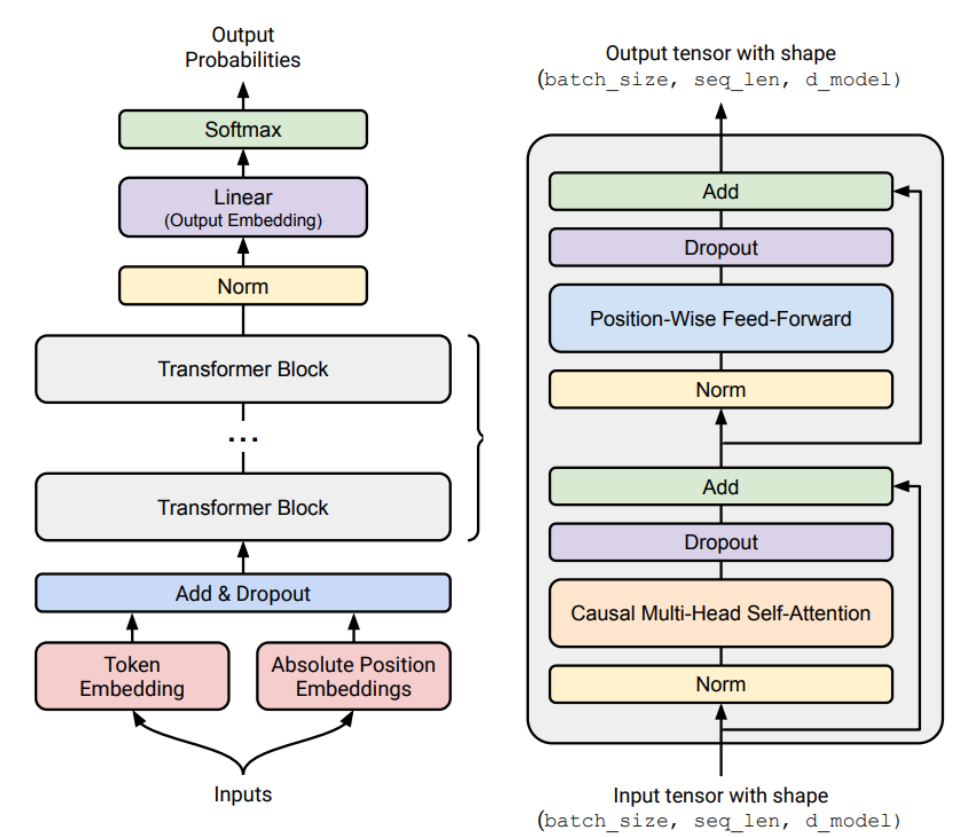
\includegraphics[width=0.86\textwidth]{../materials/spring2025-lectures/images/transformer-architecture.png}
\caption{现代语言模型虽然在细节上花样很多，但整体骨架依然围绕残差流、注意力层、前馈层与归一化层展开。}
\end{figure}

其中最强的共识来自 pre-norm。课程给出的解释并不神秘：把归一化放在 block 前面，本质上是在尽可能保留残差通路的“直通”性质，让梯度传播更稳定，也使得大模型更容易用较大的学习率训练。与之对应，post-norm 在深层模型中更容易引入训练不稳定。

\subsection{讲次 3：RMSNorm、SwiGLU 与“把不必要的参数删掉”}
CS336 对 RMSNorm 的解释很工程化：不是因为它在理论上绝对更优，而是因为它在实践中常常\textbf{足够好，而且更省数据搬运}。课程借此强调了一个会在后续系统章节反复出现的教训：少几个 FLOPs 不一定重要，但少一次不必要的 memory movement 往往很重要。

同样，SwiGLU 等 gated activation 之所以成为现代配置常客，也不是因为它们在所有设置下都严格占优，而是在大量经验中展现出更好的性能-成本平衡。第三讲因此塑造了一种非常“CS336 式”的架构观：\textbf{架构不是纯粹的美学，而是经验、规模、稳定性和系统成本共同选择的结果。}

\begin{knowledgebox}{开放权重不等于开放一切}
第三讲和第一讲一起说明了一个现实：很多现代架构细节虽然可以通过论文、代码和权重窥见一部分，但真正的训练 rationale、失败实验和调参路径通常并不完整公开。因此学习公开模型的共性，比迷信某个单独配方更重要。
\end{knowledgebox}

\subsection{讲次 4：Mixture of Experts 作为稀疏扩展}
第四讲把 MoE 放在“同等 FLOPs 下增加参数容量”的框架里理解。它的基本想法是把原本单个大前馈层替换成多个专家网络，再用路由器选择其中少数几个参与计算。这样做的诱惑非常大：\textbf{激活参数量保持较低，但总参数量可以做得很高。}

课程没有把 MoE 描述成银弹，而是明确指出它的收益来自三个方面：同 FLOPs 更高容量、训练速度可接受、并且天然适合更多设备并行；同时它也带来三类麻烦：路由与负载均衡复杂、训练目标带有启发式成分、系统实现显著更难。

从课程罗列的现实模型可以看出，今天主流 MoE 大都采用 token-choice top-k 路由，差别主要体现在 $k$ 的大小、专家粒度、是否有 shared experts，以及 load balancing 机制。DeepSeek、Qwen、Mixtral、DBRX、Grok 等公开模型的经验都指向同一个结论：\textbf{MoE 的收益不只来自“更多专家”，还来自更细粒度的设计与更成熟的系统支持。}

\begin{warningbox}{MoE 最容易被误解的地方}
MoE 不是“把参数翻十倍而 FLOPs 完全不变”的免费午餐。稀疏激活确实节省了部分计算，但路由、通信、负载不均和训练不稳定都会把理论收益打折扣，尤其是在多机环境里。
\end{warningbox}

\subsection{本章小结}
第三、四讲合起来回答的是“模型骨架应该长什么样”以及“在密集模型不够用时怎样继续扩容”。现代 Transformer 的共识部分越来越清晰，而 MoE 则代表了在固定计算预算下增加容量的主要方向之一。

\section{系统与硬件：GPU、Kernel 与并行训练}

\subsection{讲次 5：GPU 不是魔法，而是吞吐导向的机器}
第五讲从 GPU 的执行与存储层级出发，建立语言模型系统的物理直觉。CPU 擅长少量线程的低延迟执行，GPU 则擅长海量线程的高吞吐执行；SM、warp、shared memory、L2、HBM 等概念之所以重要，不是因为它们是硬件术语，而是因为它们直接决定了什么样的算法在 GPU 上会快，什么样的算法只是在“理论 FLOPs”上看起来漂亮。

\begin{figure}[H]
\centering
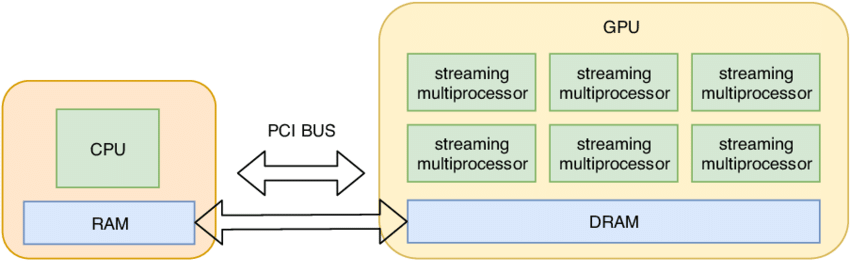
\includegraphics[width=0.82\textwidth]{../materials/spring2025-lectures/images/cpu-gpu.png}
\caption{CPU 更偏向低延迟控制流，GPU 更偏向高吞吐 SIMD/SIMT 风格执行。语言模型训练与推理之所以依赖 GPU，本质上是因为它们需要巨量并行线性代数。}
\end{figure}

课程反复强调 memory wall：算力的增长比内存带宽快得多，因此真正限制大模型速度的，经常不是“算不动”，而是“喂不饱”。这也是后面 FlashAttention、kernel fusion、低精度与并行策略一再围绕数据搬运打转的根本原因。

\subsection{讲次 6：Kernel 优化的中心任务是提高算术强度}
第六讲把很多看似零碎的优化技巧统一到了一个量上：\textbf{arithmetic intensity}，即每搬运一个字节能做多少 FLOPs。控制分支发散、低精度、operator fusion、recomputation、coalesced memory access、tiling，表面上各不相同，但本质上都在试图提高算术强度，或者至少让高算术强度部分别被低效访存拖累。

\[
I = \frac{\text{FLOPs}}{\text{Bytes Transferred}}
\]

其中：
\begin{itemize}
\item $I$：算术强度，越高说明同样的访存可以换来更多计算。
\item 分子：kernel 实际执行的浮点运算数。
\item 分母：HBM 与更近层级存储之间搬运的字节数。
\end{itemize}

Triton 在课程中扮演的是“把优化思维显性化”的工具：它逼着学生直面 tile 大小、并行布局、共享内存复用和访存模式，而不是把这些都藏在黑箱库里。CS336 想让学生明白，真正高效的 kernel 不是“写对一个公式”，而是\textbf{把数据组织成硬件喜欢的形状。}

\subsection{讲次 7：并行训练的本质是把数据、参数与状态分开切}
第七讲把大模型训练里最重要的并行原语拆开讲清：数据并行、模型并行和激活并行。其中特别关键的是 ZeRO/FSDP 系列思想：与其让每张卡冗余地保存所有参数、梯度和优化器状态，不如把这些状态按需切开、通信、聚合、释放。

\begin{figure}[H]
\centering
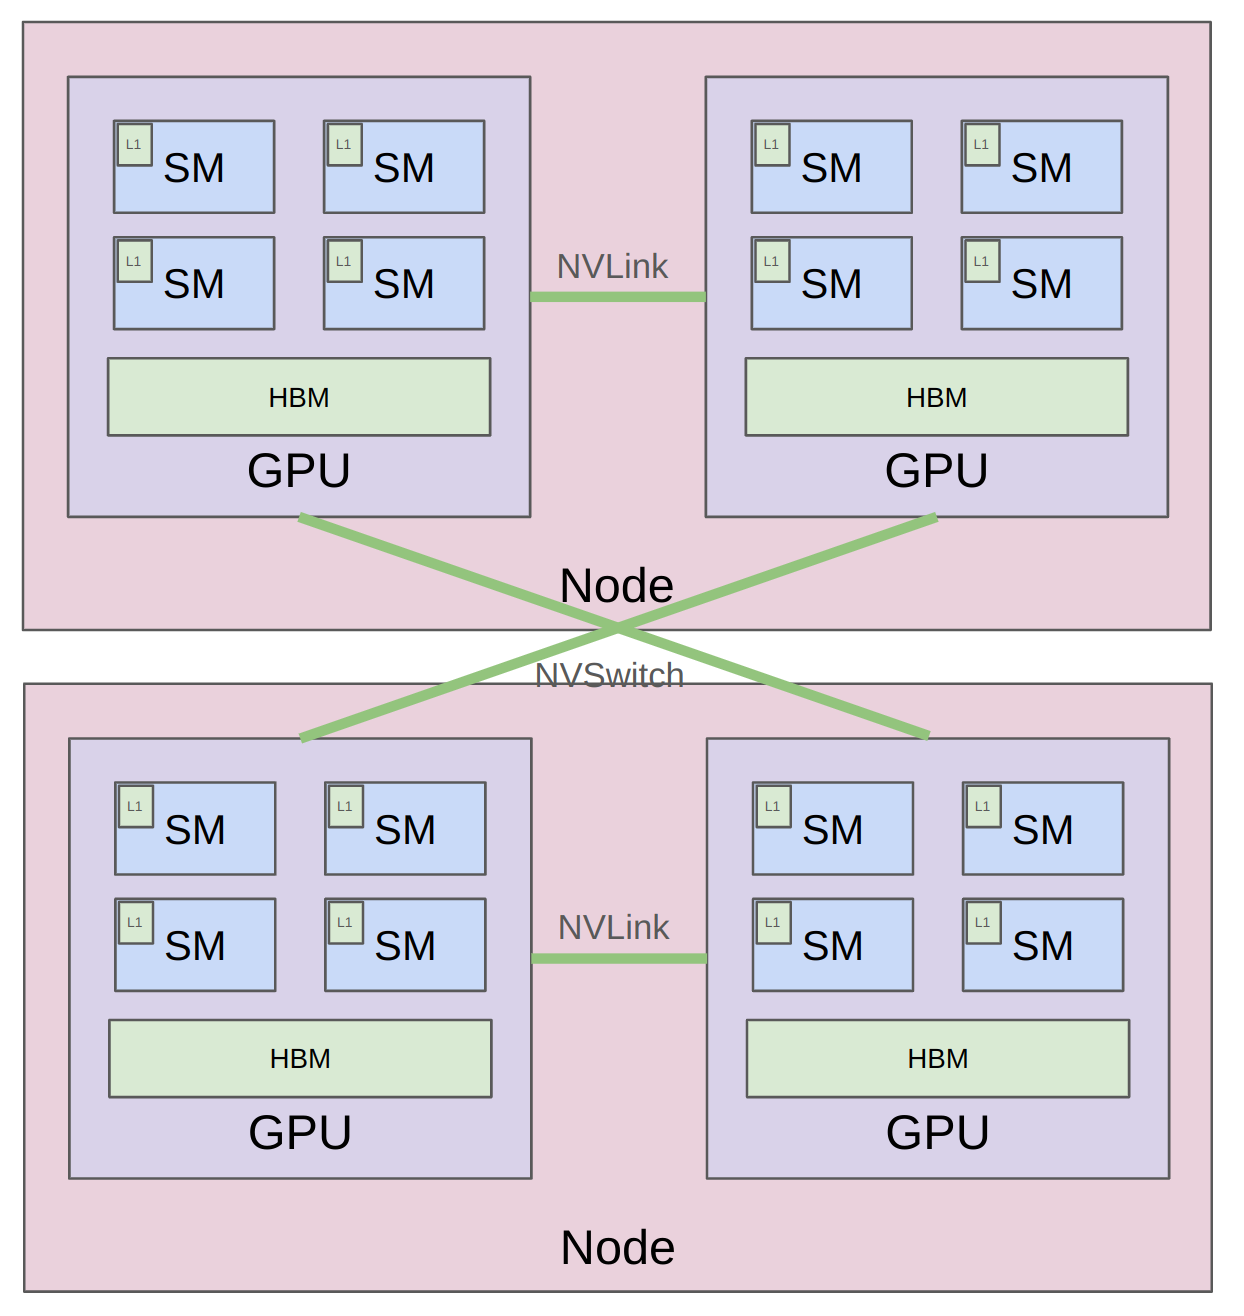
\includegraphics[width=0.82\textwidth]{../materials/spring2025-lectures/images/gpu-node-overview.png}
\caption{一旦进入多 GPU / 多机训练，单卡不再是系统的基本单位，真正的基本单位变成了整台机器乃至整个数据中心。}
\end{figure}

从课程给出的对比可以看出，ZeRO stage 1/2 的通信成本在带宽受限近似下并不比 naive DDP 更夸张，但却能显著改善内存占用；ZeRO stage 3/FSDP 更进一步把参数本身也切分出去，使超大模型能在更多 GPU 上“勉强装下”。因此并行训练不是简单的“多卡一起算”，而是\textbf{通信与存储策略的联合设计。}

\subsection{讲次 8：Collective primitives 与 distributed training 的真实基础}
第八讲把 broadcast、scatter、gather、reduce、all-gather、reduce-scatter、all-reduce 这些 collective primitive 讲得非常具体。课程的价值在于，它没有把这些 primitive 当成分布式系统教条，而是持续把它们和训练中的真实语义绑定：哪些操作用来同步梯度，哪些用来拼回参数，哪些对应 ZeRO 的 shard-update-gather 流程，哪些对应 tensor parallel 与 pipeline parallel 的激活流动。

\begin{figure}[H]
\centering
\begin{subfigure}{0.32\textwidth}
\centering
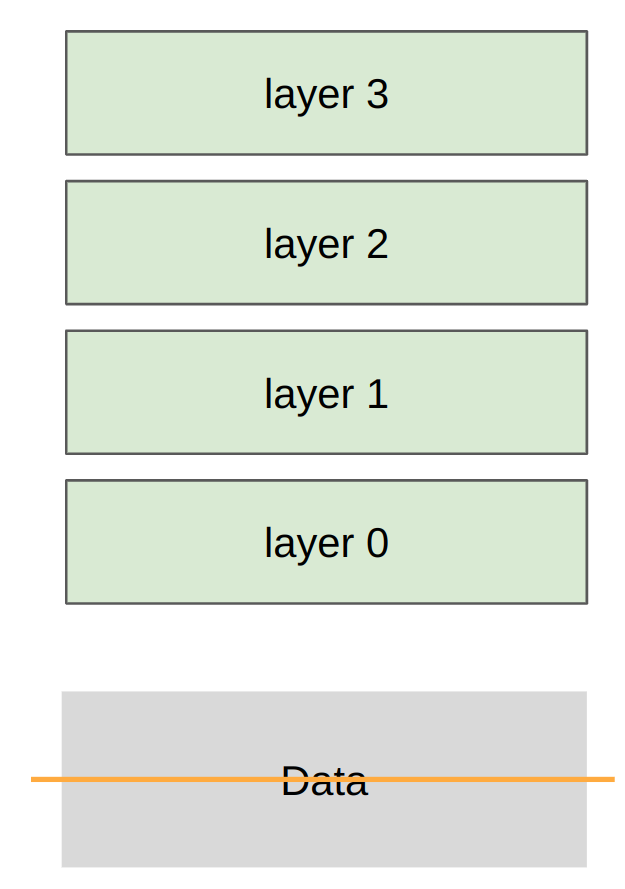
\includegraphics[width=\textwidth]{../materials/spring2025-lectures/images/data-parallelism.png}
\caption{数据并行}
\end{subfigure}
\begin{subfigure}{0.32\textwidth}
\centering
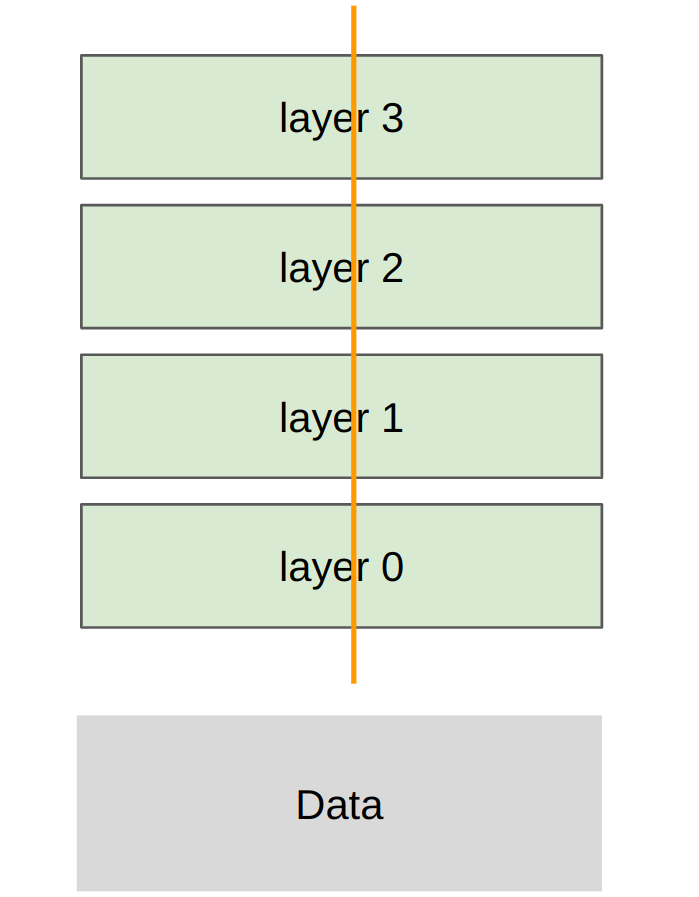
\includegraphics[width=\textwidth]{../materials/spring2025-lectures/images/tensor-parallelism.png}
\caption{张量并行}
\end{subfigure}
\begin{subfigure}{0.32\textwidth}
\centering
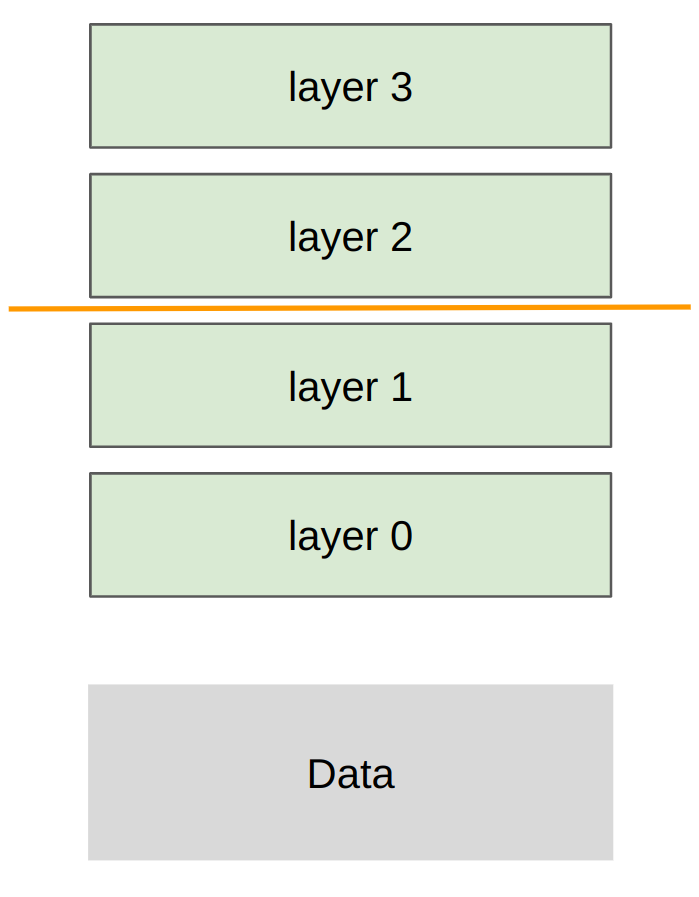
\includegraphics[width=\textwidth]{../materials/spring2025-lectures/images/pipeline-parallelism.png}
\caption{流水线并行}
\end{subfigure}
\caption{CS336 把大模型并行训练拆成几种最基本的切法：按数据切、按张量切、按层切；现实系统通常是它们的混合体。}
\end{figure}

\begin{importantbox}{系统章节的总原则}
不管是 GPU kernel 还是跨机并行，唯一不变的原则都是：\textbf{把昂贵的数据搬运变少，把不可避免的数据搬运藏到计算背后。}
\end{importantbox}

\subsection{本章小结}
第五到第八讲构成了整门课的系统内核。GPU 章节解释硬件现实，kernel 章节解释局部算子怎样贴合硬件，并行章节解释当单卡失效后如何把状态、计算与通信重新组织起来。后面所有关于训练、推理和 RL 的效率问题，都会回到这一章的直觉上。

\section{规模化方法：Scaling Laws 与训练决策}

\subsection{讲次 9：Scaling laws 为什么重要}
第九讲的问题设定非常直接：如果有人给你一万个 H100 和一个月预算，你到底该训练多大的模型、喂多少数据、如何选超参数？CS336 给出的答案不是“凭经验抄配方”，而是尽量用可外推的小规模实验来预测大规模表现，这就是 scaling laws 的方法论意义。

课程先回顾数据 scaling 的历史，再引出 Kaplan 一类神经 scaling laws 的核心观察：在 log-log 坐标里，损失与数据量、参数量、计算量之间常常呈现近似线性关系。更重要的是，这种关系不是只在语言建模里偶然出现，而是跨多个任务、多个模型家族反复出现，因此值得拿来做工程规划。

\[
L(N, D) \approx L_{\infty} + \frac{A}{N^{\alpha}} + \frac{B}{D^{\beta}}
\]

其中：
\begin{itemize}
\item $L(N,D)$：参数规模为 $N$、数据量为 $D$ 时的最终损失。
\item $L_{\infty}$：极限损失或不可约误差项。
\item $A, B$：常数项，反映模型规模与数据规模变化对损失的影响幅度。
\item $\alpha, \beta$：幂律指数，决定扩规模时收益衰减得有多快。
\end{itemize}

\begin{figure}[H]
\centering
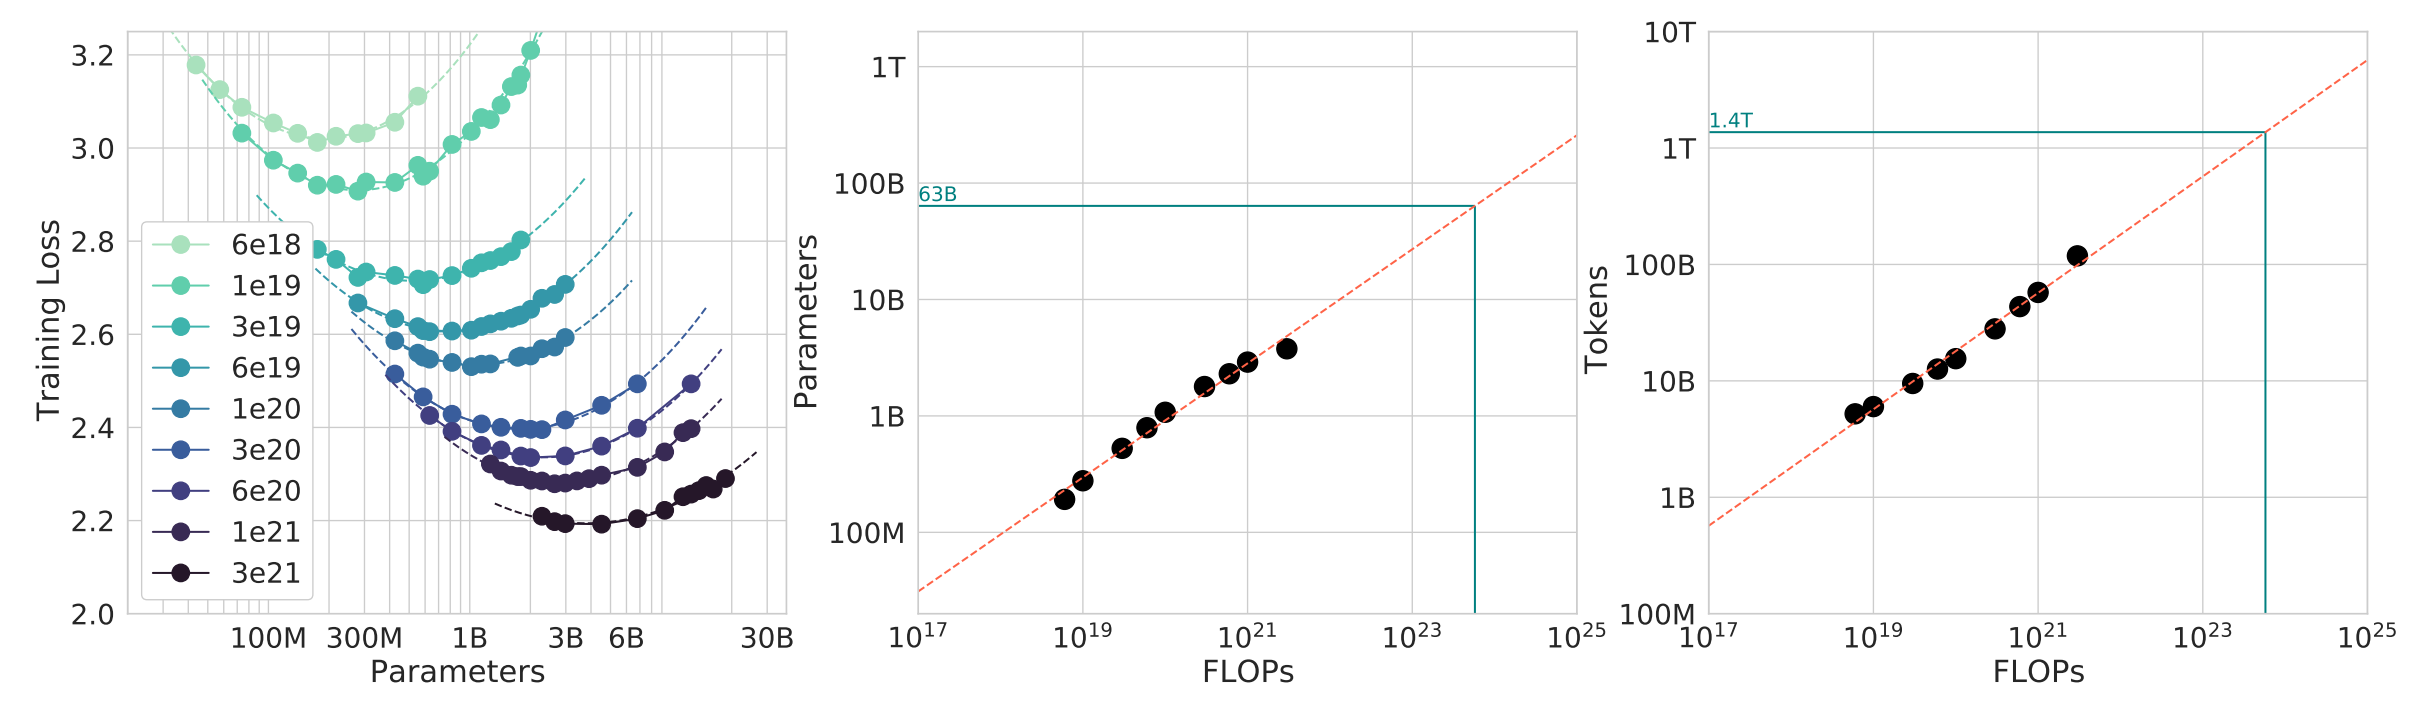
\includegraphics[width=0.72\textwidth]{../materials/spring2025-lectures/images/chinchilla-isoflop.png}
\caption{Chinchilla 式 isoflop 分析的核心，是在固定总计算预算下寻找模型参数与训练 token 的更优配比。}
\end{figure}

\subsection{讲次 9：从经验规律到训练决策}
第九讲并没有把 scaling laws 神化为自然定律，而是把它当成\textbf{预算分配器}。在固定 FLOPs 预算下，你可以把算力花在更大的模型上，也可以花在更长的训练上；没有 scaling laws，这个决策只能靠粗糙经验；有了 scaling laws，你至少可以在小规模上拟合出可参考的趋势，再决定大规模试验怎么做。

课程也特别提醒，经典统计学习里常见的 $1/n$ 误差直觉，并不能直接解释神经网络中观察到的 exponent。也就是说，scaling laws 的经验有效性很强，但它们背后的理论解释仍不完全闭合。这种“强工程价值、弱理论定案”的状态，正是现代大模型研究的典型特征。

\subsection{讲次 11：现代 scaling recipe 已经比 Chinchilla 更复杂}
第十一讲把视角从 2020--2022 年的基础结论，推进到 2024--2025 年的现代 recipe。CerebrasGPT、MiniCPM、DeepSeek、LLaMA 3、Hunyuan、MiniMax 等公开实践共同说明：今天的 scaling recipe 不再只是简单套用“$20 \times$ 参数量”这条经验，而是把 \textbf{muP、批大小、学习率、学习率调度和 isoflop 分析} 一起纳入。

课程尤其强调两类技术。第一类是 \textbf{muP}，它试图让不同宽度模型之间的超参数调优更具有尺度不变性，从而把大模型超参数搜索尽可能搬回小模型阶段。第二类是 \textbf{WSD} 之类的学习率调度，它让人能在不完整跑满所有训练曲线的情况下，仍然比较便宜地拟合出近似 Chinchilla 风格的最优配比。

\begin{figure}[H]
\centering
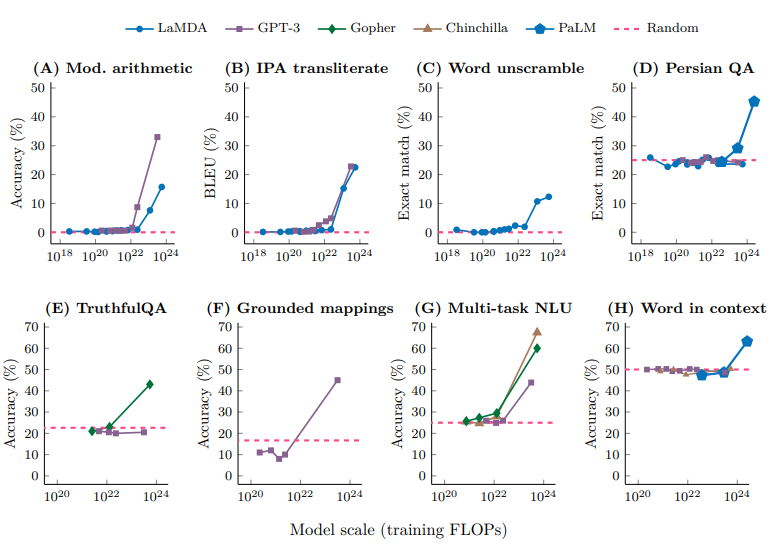
\includegraphics[width=0.66\textwidth]{../materials/spring2025-lectures/images/wei-emergence-plot.png}
\caption{规模增长并不只带来平滑收益，也常伴随“某些能力突然变得可见”的现象，这也是简单从小模型直觉外推到大模型时最需要小心的地方。}
\end{figure}

\begin{warningbox}{Scaling law 的使用边界}
不要把 scaling law 当成不可违背的物理常数。它们强在资源规划与趋势预测，弱在对架构变化、数据分布变化、目标函数变化的鲁棒性。配方一旦换了，拟合就要重新做。
\end{warningbox}

\subsection{本章小结}
第九和第十一讲共同确立了 CS336 的规模化视角：大模型训练不应该靠运气和 cargo cult，而应该通过小规模实验拟合大规模趋势，再把预算投到最可能有效的方向上。与此同时，现代实践也说明 scaling recipe 本身仍在快速演化。

\section{推理系统：Prefill/Decode、KV Cache 与低成本近似}

\subsection{讲次 10：推理与训练是两种不同的工作负载}
第十讲的最大贡献，是把“模型已经训完”之后的系统问题完整摊开。课程强调，推理并不是训练的简化版。训练的主要目标是高吞吐地处理大量已知 token，而推理尤其是生成阶段，必须逐 token 串行展开，因此它更容易成为 memory-bound workload。

CS336 用三个在线服务指标来组织推理问题：TTFT（首 token 时延）、latency（每 token 延迟）和 throughput（整体吞吐）。这三个指标之间并不完全一致：提高 batch size 可能能提高吞吐，但也会恶化单请求时延；共享前缀和动态到达流量又会进一步破坏“整齐批处理”的理想设定。

\subsection{讲次 10：Prefill 与 Decode 的本质差异}
课程把推理拆成 prefill 和 decode 两个阶段。prefill 阶段给定完整 prompt，可以像训练一样并行处理整段输入，因此更容易达到 compute-bound；decode 阶段每次只生成一个新 token，MLP 与 attention 都更难获得足够高的算术强度，特别是 attention 几乎不从批量中受益。

\begin{figure}[H]
\centering
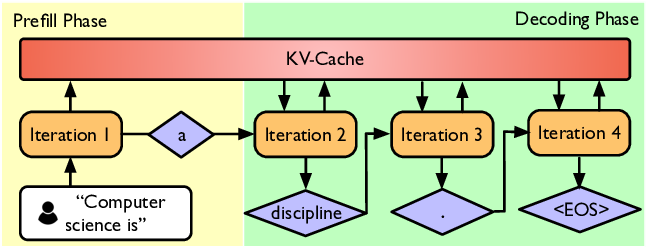
\includegraphics[width=0.78\textwidth]{../materials/spring2025-lectures/images/prefill-decode.png}
\caption{Prefill 更像并行编码，decode 更像不断读取历史状态并做小步递推；两者的系统瓶颈完全不同。}
\end{figure}

这也是 KV cache 成为现代推理系统核心组件的原因。没有 KV cache，生成 $T$ 个 token 的成本会重复扫描历史前缀；有了 KV cache，前缀工作得以复用，但新的问题转变成：\textbf{如何高效存、取、共享和分页这些缓存。}

\subsection{讲次 10：为了更快推理，可以改哪里}
课程把推理优化分成几类。第一类是\textbf{改架构}，包括 GQA、MLA、局部注意力、状态空间模型等，它们试图从根本上减轻 KV cache 或 attention 的成本。第二类是\textbf{改数值表示}，如量化、低比特权重表示。第三类是\textbf{改执行流程}，如 speculative decoding、continuous batching 与 paged attention。

\begin{figure}[H]
\centering
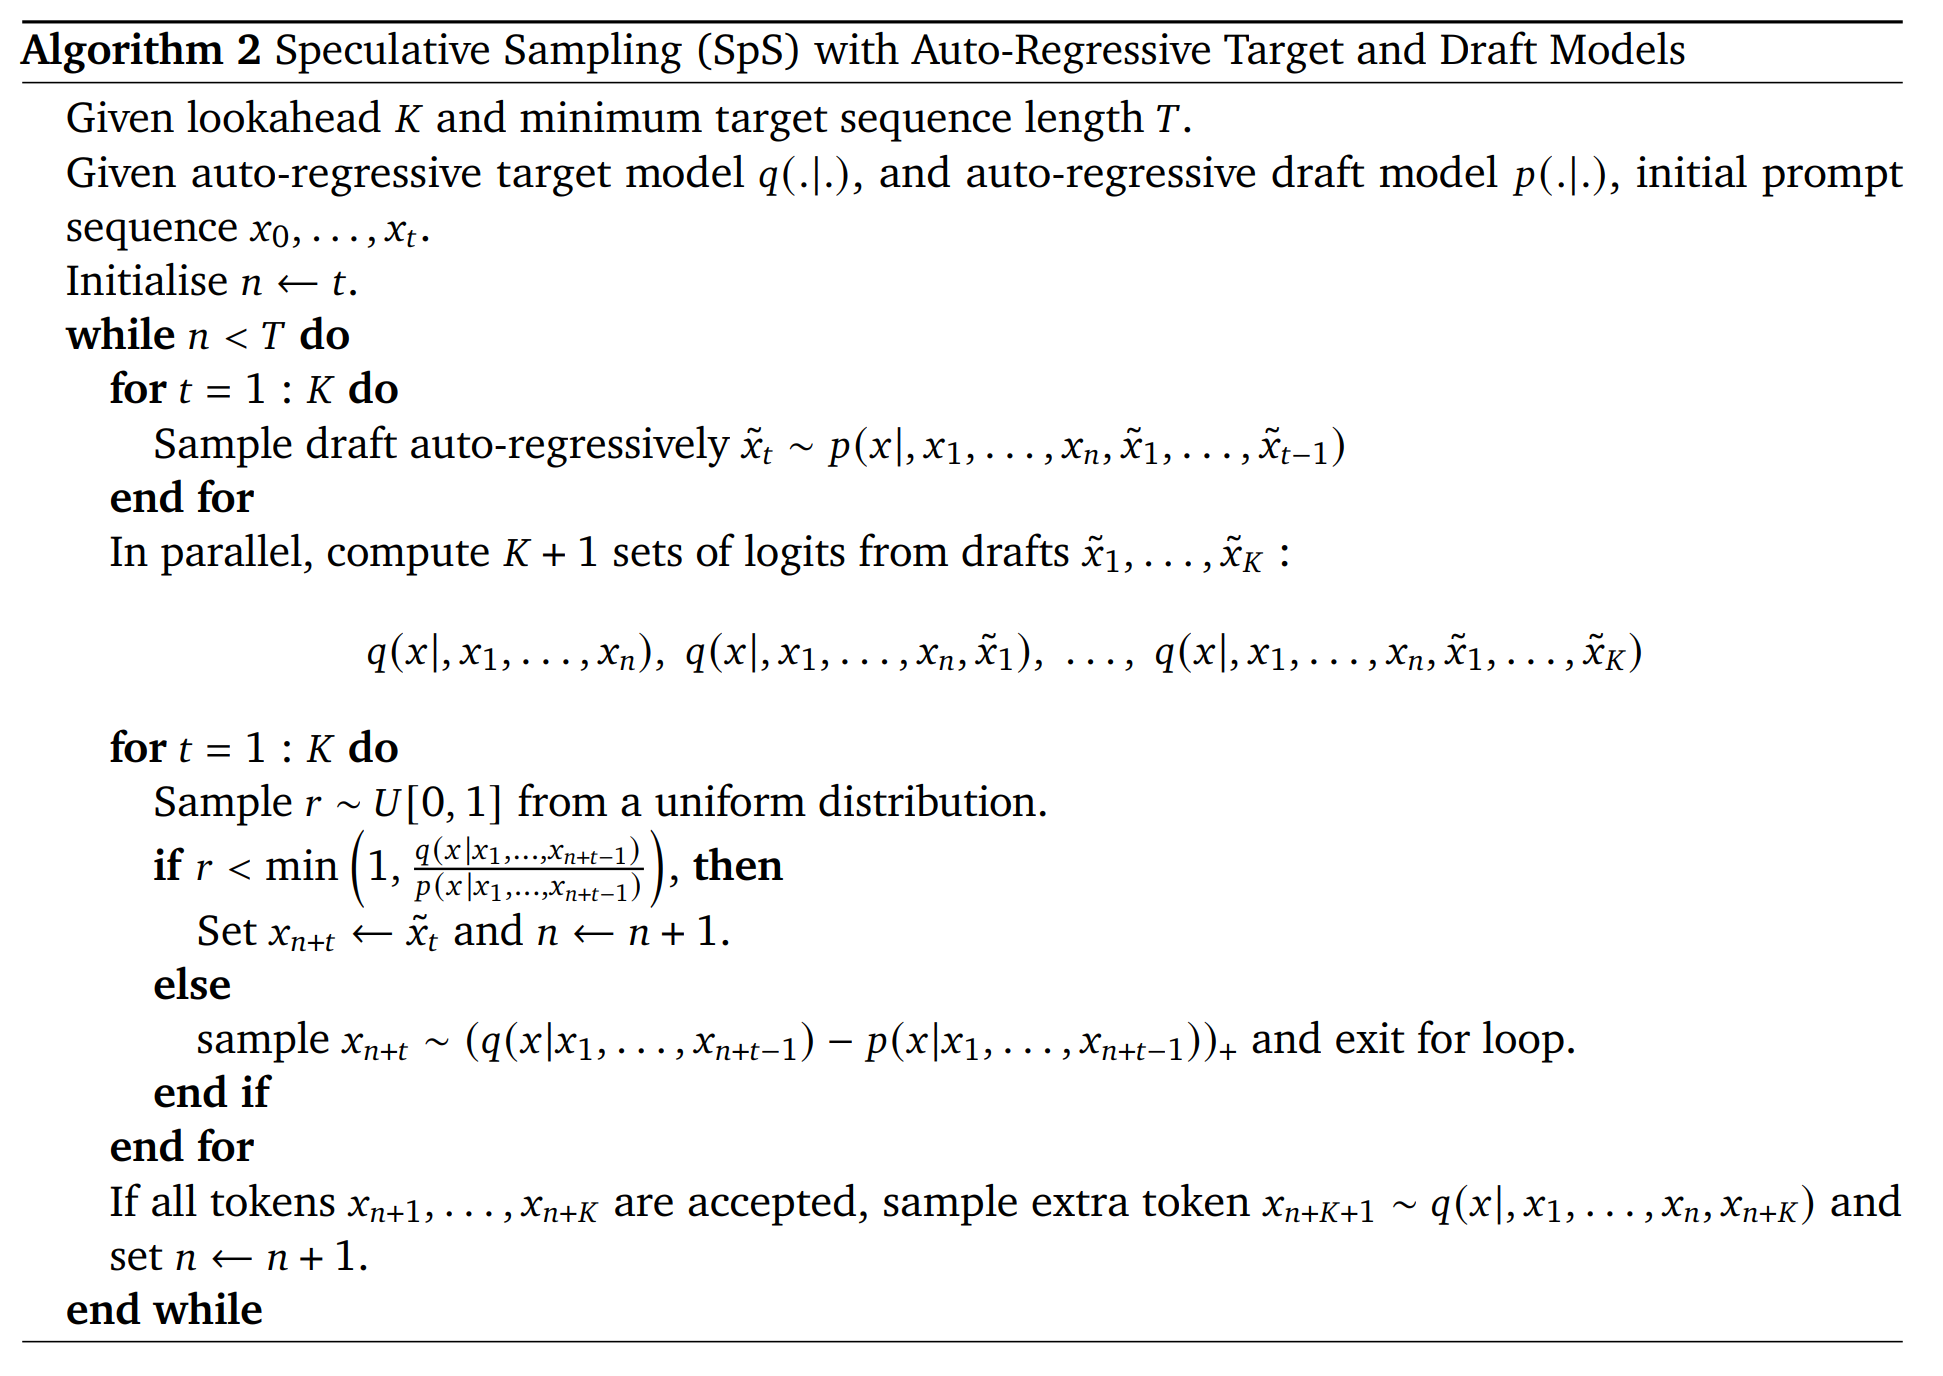
\includegraphics[width=0.74\textwidth]{../materials/spring2025-lectures/images/speculative-sampling-algorithm.png}
\caption{Speculative decoding 的关键思想是：先用便宜模型提案，再用大模型并行验证，从而用近似流程换取精确输出下的系统加速。}
\end{figure}

\begin{figure}[H]
\centering
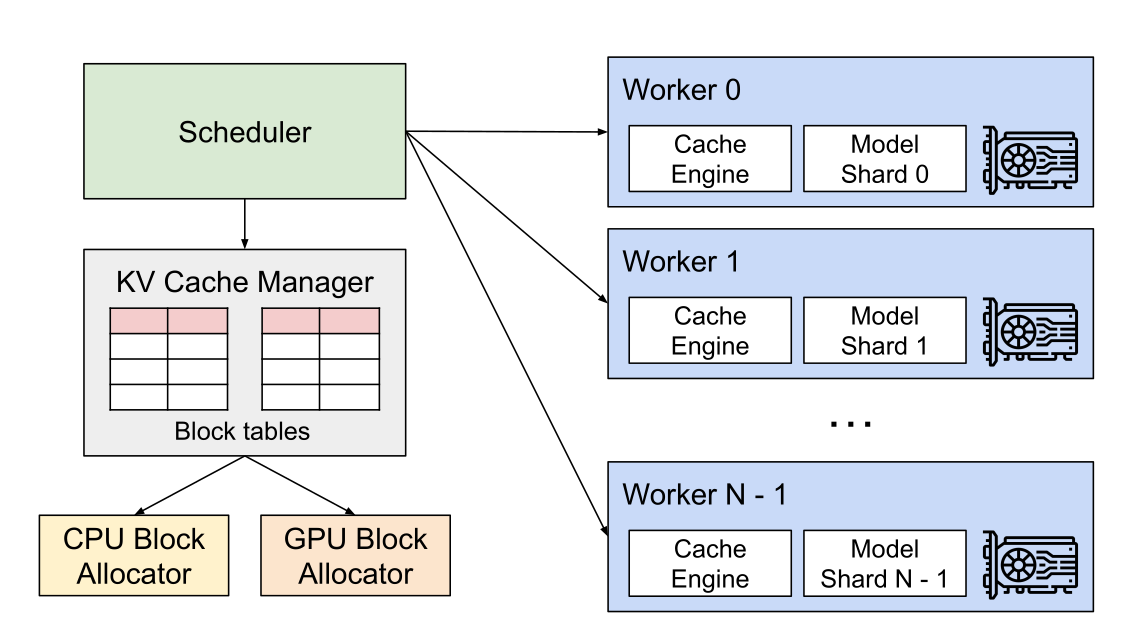
\includegraphics[width=0.72\textwidth]{../materials/spring2025-lectures/images/paged-attention-vllm.png}
\caption{Paged attention 把 KV cache 变成更灵活的块式管理对象，使动态批处理、共享前缀和不同长度请求能在一个统一的内存抽象里共存。}
\end{figure}

\subsection{讲次 10：准确率与速度之间没有白拿的便宜}
第十讲一直在提醒一点：很多加速技巧都是“lossy shortcut”。GQA、MLA、量化、剪枝、蒸馏都会改变模型本身；speculative decoding 与 paged attention 则更多是在不改语义结果的前提下优化执行过程。课程因此把推理优化分成两种心智模型：\textbf{可以牺牲一点能力换取更低成本}，以及\textbf{不改变答案但重写执行方式}。

\subsection{本章小结}
第十讲把推理系统从“部署时顺手做一下”提升成课程核心内容之一。它说明了为什么 decode 阶段天然困难，为什么 KV cache 是中心对象，以及为什么现代推理优化会同时涉及架构、数值表示与系统执行三条线。

\section{评估与数据工程}

\subsection{讲次 12：评估不是一个分数，而是一整套任务分解}
第十二讲系统梳理了语言模型评估的谱系。从最传统的 perplexity，到 MMLU、GPQA、HLE 这类知识与推理 benchmark，再到 AlpacaEval、IFEval、WildBench、Chatbot Arena、SWE-Bench、CyBench、MLEBench 等更接近真实使用的评估，课程想强调的是：\textbf{“模型强不强” 不是单一维度。}

\begin{figure}[H]
\centering
\begin{subfigure}{0.48\textwidth}
\centering
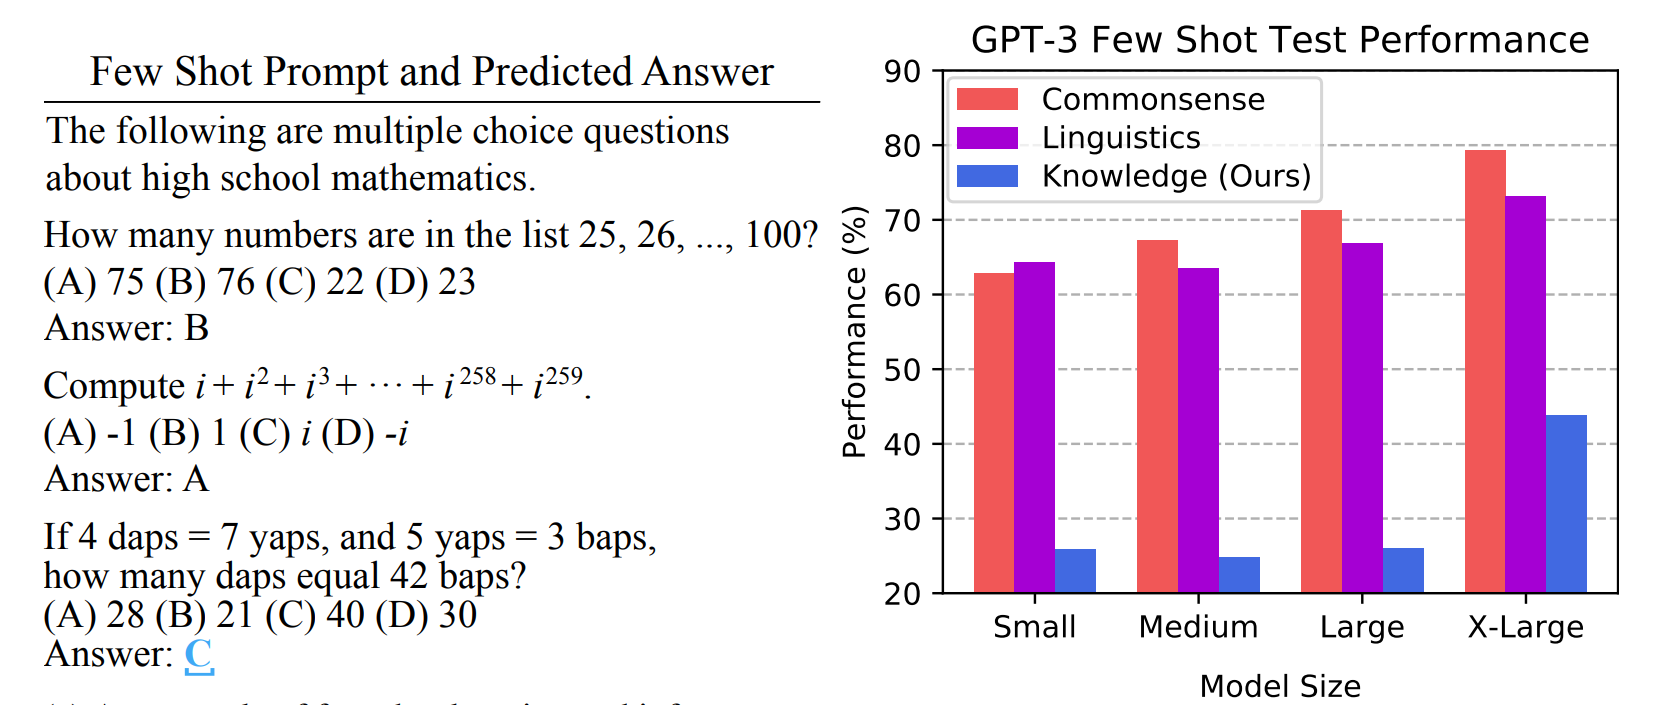
\includegraphics[width=\textwidth]{../materials/spring2025-lectures/images/mmlu.png}
\caption{MMLU 一类标准化测试}
\end{subfigure}
\begin{subfigure}{0.48\textwidth}
\centering
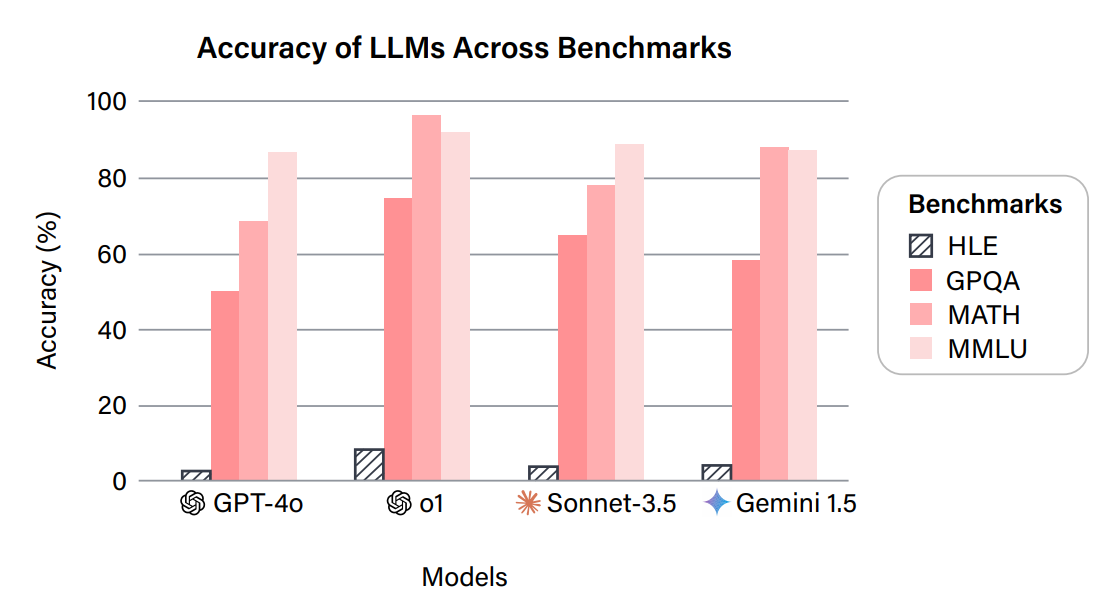
\includegraphics[width=\textwidth]{../materials/spring2025-lectures/images/hle-results.png}
\caption{更高难度综合评估}
\end{subfigure}
\caption{从标准学科题到更高层次综合测试，评估维度在不断扩展。}
\end{figure}

CS336 在这里给出的重要经验是：benchmark score 与真实用户感受之间并不总是一一对应。风格偏好、长度偏置、judge bias、任务构造方式、是否允许 test-time compute，都会深刻影响结论。因此评估章节本质上是在教学生\textbf{如何怀疑分数、如何拆解分数背后的生成机制。}

\subsection{讲次 13：数据不是“抓下来就能训”的原料}
第十三讲把数据问题拉回现实世界。课程先从预训练数据来源讲起：网页、书籍、论文、代码仓库等原始材料，并指出真正困难的不是“来源很多”，而是它们格式复杂、质量差异大、法律地位不同，而且不同使用阶段的风险也不同。

课程对版权、license、fair use、terms of service 的讨论尤其重要。它并不提供简单的“一刀切合法性结论”，而是提醒学生：数据工程从来不只是技术处理，还是一种合规与风险管理问题。对大模型工程而言，\textbf{能不能用某份数据，和怎样把它变成可训练语料，同样重要。}

\subsection{讲次 14：数据处理的关键是过滤、去重与预算分配}
第十四讲进一步进入真正的数据工程细节：网页转文本、质量过滤、去重、重复数据的边际价值、数据混合比例、如何用小规模实验判断哪类数据更值得保留。课程把 CCNet、fastText 分类器、Jaccard 相似度、MinHash 等方法摆到一起，目的不是教具体工具，而是让学生理解：\textbf{数据质量本身就是算力效率。}

\begin{figure}[H]
\centering
\begin{subfigure}{0.48\textwidth}
\centering
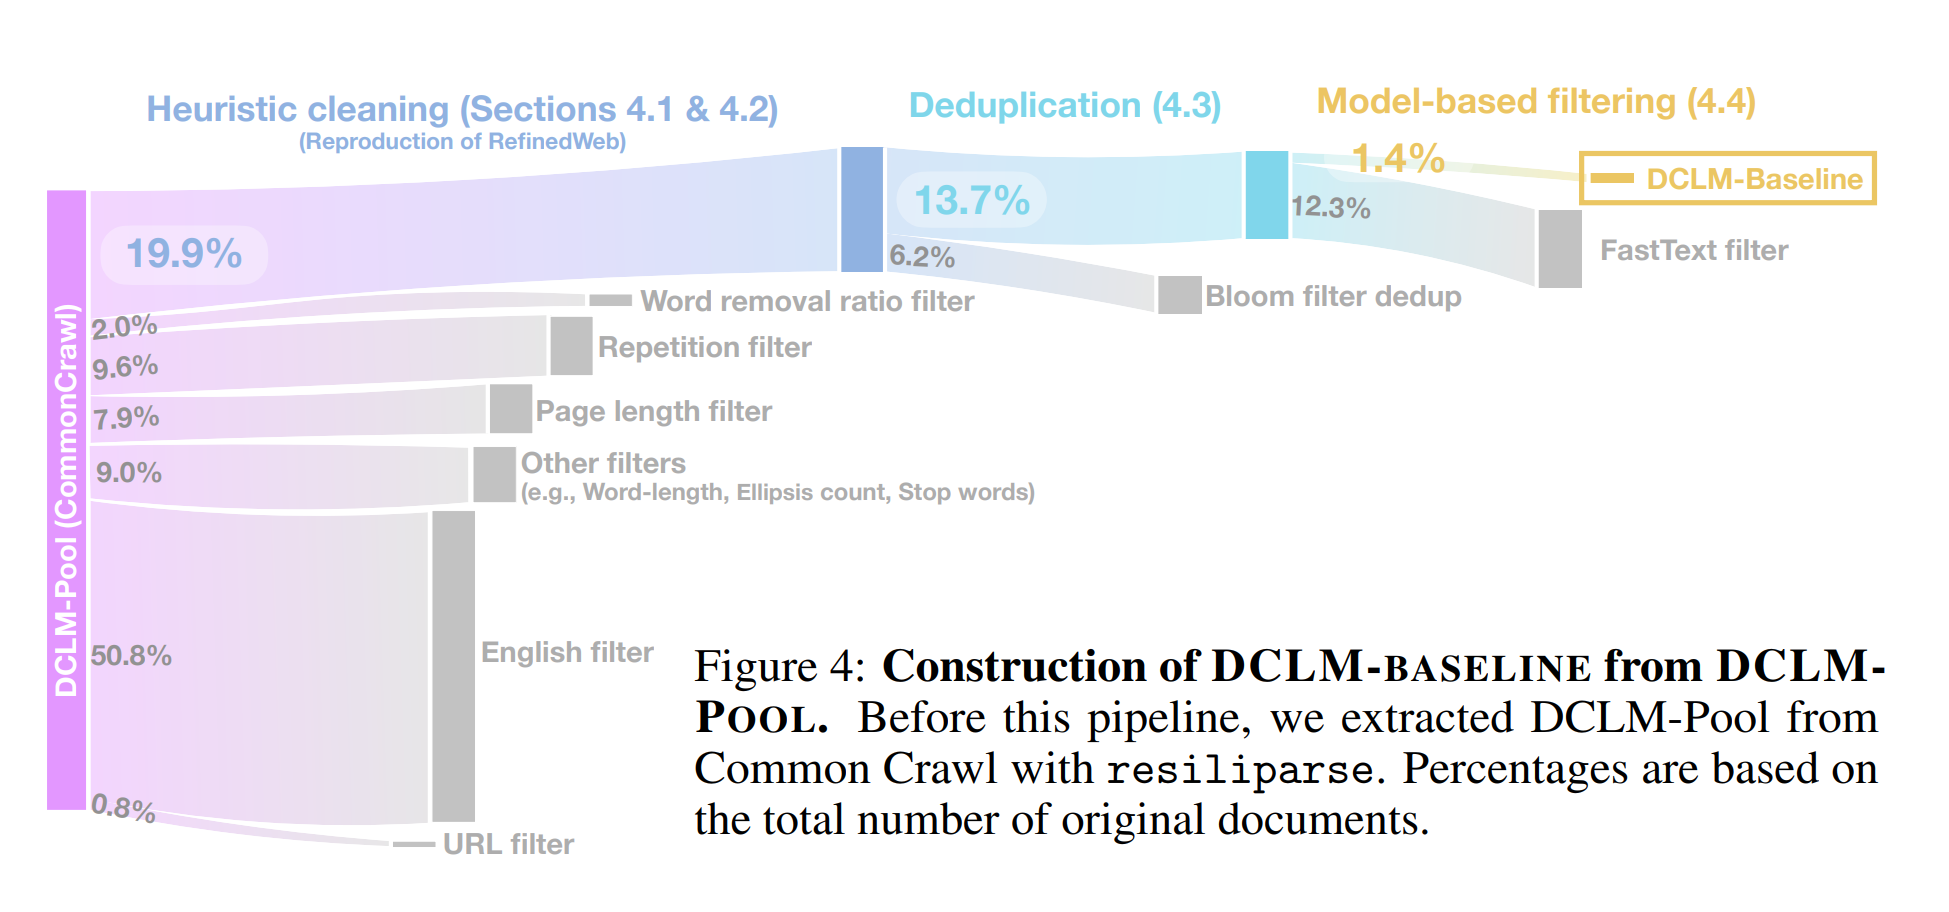
\includegraphics[width=\textwidth]{../materials/spring2025-lectures/images/dclm-filter.png}
\caption{质量过滤}
\end{subfigure}
\begin{subfigure}{0.48\textwidth}
\centering
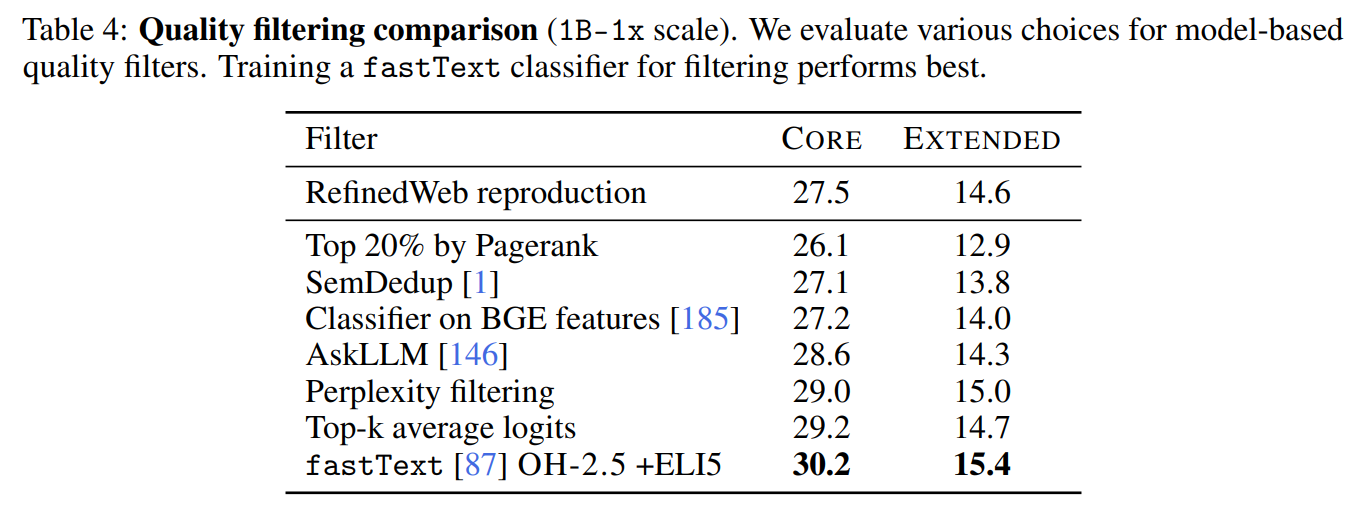
\includegraphics[width=\textwidth]{../materials/spring2025-lectures/images/dclm-quality.png}
\caption{质量与效果关系}
\end{subfigure}
\caption{高质量数据不会凭空出现，需要经过转换、过滤、去重与混配。}
\end{figure}

\begin{importantbox}{数据章节的压缩结论}
在算力紧缺时代，训练在坏数据上的每一步优化，都是对预算的浪费。数据工程并不是训练前的“杂活”，而是直接决定最终 perplexity 与下游能力的主战场。
\end{importantbox}

\subsection{本章小结}
评估章节教我们如何判断模型能力，数据章节教我们如何塑造模型能力。前者避免“被分数骗”，后者避免“把算力花在不值得的样本上”。两者合在一起，构成了训练闭环中最容易被低估、但最难靠蛮力补救的部分。

\section{对齐：从 SFT/RLHF 到 RLVR}

\subsection{讲次 15：为什么预训练模型还不够}
第十五讲把“base model 很强”与“assistant model 真正可用”之间的差距讲得非常清楚。预训练擅长学会继续文本分布，但真实使用场景要求模型更好地遵循指令、控制风格、维持安全边界，甚至在特定场景下展现更稳定的格式与行为。因此，仅靠预训练并不能自然得到 InstructGPT 一类助手模型。

课程把标准路线概括为 imitation 加 reinforcement：先做 SFT，再做 RLHF。SFT 的核心不是“拿一些问答数据再训一遍”这么简单，而是要关注数据里面到底教给模型什么：仅仅是任务答案，还是回答长度、口吻、引用方式、格式结构与安全行为。

\subsection{讲次 15：SFT 数据的真正难点在于它改变了模型行为分布}
CS336 用 FLAN、Alpaca、OpenAssistant 等数据例子说明，不同 instruction 数据集在长度、项目符号风格、引用、知识复杂度和安全性方面差异极大。这意味着 SFT 不只是向模型注入“新知识”，更是在重塑模型面对 prompt 时的默认行为模式。

\begin{warningbox}{SFT 不是免费知识注入}
课程特别提醒：把模型不太会的尾部知识直接拿去微调，未必会得到更可靠的知识行为，反而可能诱发新的幻觉模式。SFT 更擅长塑造行为边界，而不是稳健地重写底层知识库。
\end{warningbox}

\subsection{讲次 16：从 DPO 到 PPO，再到 GRPO 的动机}
第十六讲先回顾 DPO 的核心思想：在一些合理假设下，可以把 RLHF 问题转写成基于偏好对的监督式目标，从而避免 PPO 中 reward model、rollout 与 value function 带来的不少工程复杂性。课程也强调，DPO 之所以广受欢迎，不是因为它在所有问题上都赢，而是因为它\textbf{大幅降低了做对齐实验的系统门槛。}

但当数据并非天然成对比较，或者我们希望利用可验证奖励直接在线优化时，PPO / GRPO 一类方法仍然会回来。PPO 的问题在于实现复杂、value model 昂贵、调参与稳定性负担很重；GRPO 的出现，则是在语言模型这个“同一 prompt 下能自然采样多个回答”的场景中，利用组内标准化奖励替代显式 critic。

\[
\nabla_{\theta} \mathbb{E}[R] = \mathbb{E}\left[\nabla_{\theta}\log \pi_{\theta}(a \mid s)\, R(s,a)\right]
\]

其中：
\begin{itemize}
\item $s$：状态，这里可以理解为 prompt 加上当前已生成前缀。
\item $a$：动作，在语言模型场景里可以是整段回答，也可以是逐 token 动作序列。
\item $\pi_{\theta}(a \mid s)$：参数为 $\theta$ 的策略，也就是当前语言模型。
\item $R(s,a)$：奖励，可能来自偏好模型，也可能来自可验证程序。
\end{itemize}

\subsection{讲次 17：Baseline、Advantage 与 GRPO 的机械细节}
第十七讲把 policy gradient 的核心机械结构彻底拆开。最原始的更新形式直接拿奖励乘以 log-prob 梯度，但方差太大；因此需要 baseline，把“同一个 prompt 下平均能拿到多少回报”减掉，只保留“这次回答比平均水平更好还是更差”的部分，也就是 advantage。

在语言模型场景里，这种 baseline 有天然的组结构：同一个 prompt 下生成多条回答，就能直接用组内均值甚至组内标准差做归一化，从而得到 GRPO 的简化目标。课程用排序任务的小例子说明，哪怕目标函数本身很简单，reward 形状、baseline 选取、clipping 与 KL 正则也会显著改变训练动态。

\begin{figure}[H]
\centering
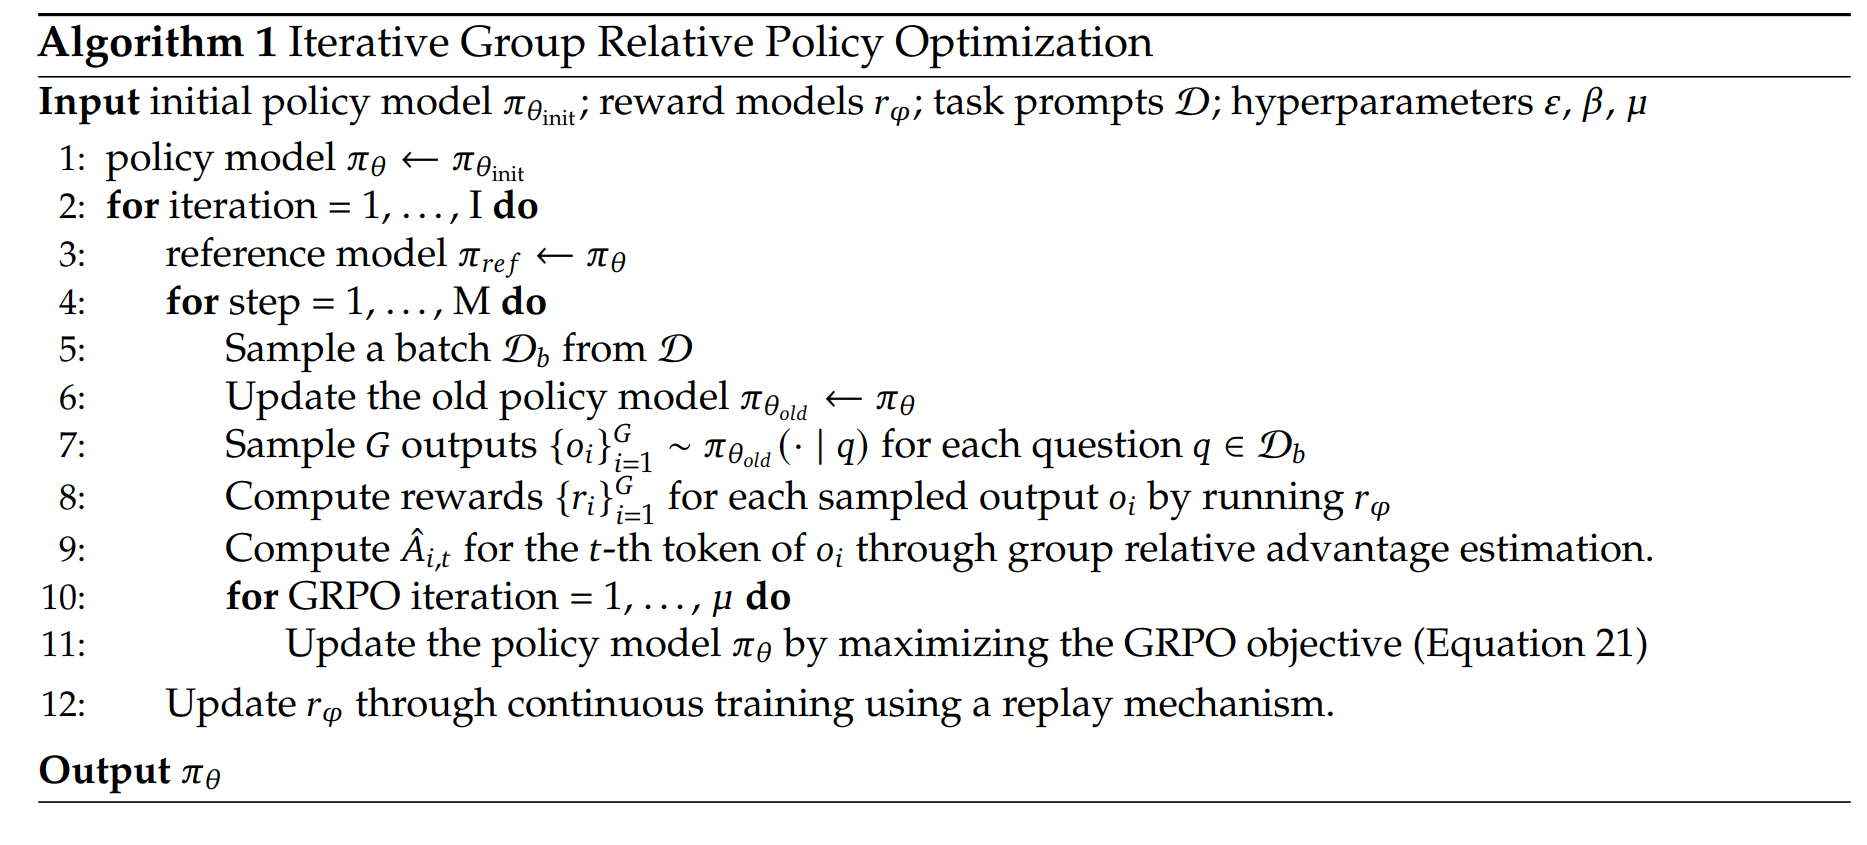
\includegraphics[width=0.74\textwidth]{../materials/spring2025-lectures/images/grpo-algorithm.png}
\caption{GRPO 可以看成去掉 critic 后、依赖组内奖励归一化的 PPO 近亲：实现更轻，但稳定性和效果仍高度依赖 reward 设计与训练细节。}
\end{figure}

\begin{lstlisting}[caption={极简的组内归一化策略梯度伪代码}]
responses = model.sample(prompts, group_size=G)
rewards = verifier(responses)
advantages = (rewards - rewards.mean(dim=1, keepdim=True)) / (
    rewards.std(dim=1, keepdim=True) + 1e-4
)
loss = -(advantages.detach() * logprob_ratio_clipped).mean()
\end{lstlisting}

\subsection{讲次 16--17：RLVR 为什么把课程终点推到了 o1 / r1 时代}
CS336 对 RLVR 的理解非常务实。传统 RLHF 的奖励往往来自偏好或 judge，因此容易受过优化、模式坍塌和 reward hacking 影响；而在数学、代码、形式逻辑等可验证场景中，如果奖励可以更接近“对就是对，错就是错”，那强化学习就有更大的机会把模型往真正更强的方向推。

这也是课程从 ``GPT-3 $\rightarrow$ GPT-3.5'' 一路推到 ``o1 / r1'' 的逻辑：不是单纯靠更大的预训练规模，而是靠\textbf{更好的推理时计算、更强的反馈信号，以及更会被优化的目标函数。}

\subsection{本章小结}
对齐模块完成了从 imitation 到 reinforcement 的闭环。SFT 教模型学会像助手那样说话，DPO 提供了更低摩擦的偏好优化路径，PPO 与 GRPO 则把我们带到在线优化和可验证奖励的世界。课程最终想说明的是：可控性和推理能力，并不是预训练的附属物，而是后训练时代的主战场。

\section{总结与延伸}
把整门 CS336 串起来看，可以把语言模型的构建过程压缩成四句话。

第一，\textbf{语言模型不是单个网络，而是一套资源分配系统。} Tokenization、架构、优化器、数据处理、推理系统与后训练都在争夺同一份预算。只有把这些决策统一起来，才会真正明白“从零构建”意味着什么。

第二，\textbf{系统效率决定了哪些算法在现实里有意义。} 课程从 GPU、kernel、并行通信到推理系统，不断说明：现代大模型的很多“算法创新”，本质上都是为了减少数据搬运、提高算术强度、降低状态冗余，或者让更多计算预算落到真正有价值的地方。

第三，\textbf{规模化不是盲目堆大，而是用规律规划预算。} scaling laws、muP、WSD、isoflop 分析之所以重要，并不是因为它们能给出永远正确的答案，而是因为它们让大规模试验不再完全依赖拍脑袋。

第四，\textbf{后训练决定模型最终能否变成可用系统。} 预训练给模型潜力，评估告诉我们它哪里强哪里弱，数据工程决定我们把什么喂进模型，而 SFT、DPO、PPO、GRPO 与 RLVR 则负责把这种潜力转化成更可控、更可靠、甚至更会推理的行为。

\begin{importantbox}{整门课的压缩结论}
如果只能记住一句话，那么应该是：\textbf{构建语言模型，就是在真实资源约束下，把数据、表示、架构、系统与反馈信号联合优化。}
\end{importantbox}

从后续学习路径看，这门课之后最值得继续深挖的方向有三个：一是更强的数据治理与合规实践，二是更成熟的推理系统与 serving 框架，三是把可验证奖励和 test-time compute 结合起来的新一代后训练方法。前沿模型的竞争，正越来越集中在这三条线上。

\end{document}
